%\section{Written Questions}

%%%%%%%%%%%%%%%%%%%%%%%%%%%%%%%%%%%%%%%%%%%%%
% Q1
%%%%%%%%%%%%%%%%%%%%%%%%%%%%%%%%%%%%%%%%%%%%%
\begin{question}[1. Insertion Sort]{
Implement \code{insertion_sort(…)} in \code{sort.c}.
}
%\begin{answer}
\begin{lstlisting}[language=C, style=C]
void insertion_sort(int arr[], int low, int high)
{
    for (int i = low + 1; i < high; i++) {
        int key = arr[i];
        int j = i - 1;
        while (j >= low && arr[j] > key) {
            arr[j + 1] = arr[j];
            j--;
        }
        arr[j + 1] = key;
    }
}
\end{lstlisting}
%\end{answer}
\end{question}


%%%%%%%%%%%%%%%%%%%%%%%%%%%%%%%%%%%%%%%%%%%%%
% Q2
%%%%%%%%%%%%%%%%%%%%%%%%%%%%%%%%%%%%%%%%%%%%%
\begin{question_with_subs}[2. Merge Sort]{}
%%%%% A %%%%%
\begin{subq}{Implement \code{merge(…)} in \code{sort.c}.}
\begin{lstlisting}[language=C, style=C]
void merge(int arr[], int low, int mid, int high)
{
    int n1 = mid - low;
    int n2 = high - mid;

    int* left = (int*)malloc(sizeof(int) * n1);
    int* right = (int*)malloc(sizeof(int) * n2);

    for (int i = 0; i < n1; i++)
        left[i] = arr[low + i];
    for (int j = 0; j < n2; j++)
        right[j] = arr[mid + j];

    int i = 0, j = 0, k = low;
    while (i < n1 && j < n2) {
        if (left[i] <= right[j]) {
            arr[k++] = left[i++];
        } else {
            arr[k++] = right[j++];
        }
    }
    while (i < n1)
        arr[k++] = left[i++];
    while (j < n2)
        arr[k++] = right[j++];

    free(left);
    free(right);
}
\end{lstlisting}
\end{subq}

%%%%% B %%%%%
\begin{subq}{Implement \code{merge_sort(…)} in \code{sort.c.}}
\begin{lstlisting}[language=C, style=C]
void merge_sort(int arr[], int low, int high)
{
    if (high - low <= 1) return;
    int mid = low + (high - low) / 2;
    merge_sort(arr, low, mid);
    merge_sort(arr, mid, high);
    merge(arr, low, mid, high);
}
\end{lstlisting}
\end{subq}
\end{question_with_subs}


%%%%%%%%%%%%%%%%%%%%%%%%%%%%%%%%%%%%%%%%%%%%%
% Q3
%%%%%%%%%%%%%%%%%%%%%%%%%%%%%%%%%%%%%%%%%%%%%
\begin{question_with_subs}[3. Quick Sort]{}
%%%%% A %%%%%
\begin{subq}{Implement \code{partition(…)} in \code{sort.c}.}
\begin{lstlisting}[language=C, style=C]
int partition(int arr[], int low, int high)
{
	int pivot_index = low + rand() % (high - low);
    swap(&arr[pivot_index], &arr[high - 1]);
    int pivot = arr[high - 1];
    int i = low - 1;
    for (int j = low; j < high - 1; j++) {
        if (arr[j] <= pivot) {
            i++;
            swap(&arr[i], &arr[j]);
        }
    }
    swap(&arr[i + 1], &arr[high - 1]);
    return i + 1;
}
\end{lstlisting}
\end{subq}

%%%%% B %%%%%
\begin{subq}{Implement \code{quick_sort(…)} in \code{sort.c.}}
\begin{lstlisting}[language=C, style=C]
void quick_sort(int arr[], int low, int high)
{
    if (low < high - 1) {
        int p = partition(arr, low, high);
        quick_sort(arr, low, p);
        quick_sort(arr, p + 1, high);
    }
}
\end{lstlisting}
\end{subq}
\end{question_with_subs}


\newpage

%%%%%%%%%%%%%%%%%%%%%%%%%%%%%%%%%%%%%%%%%%%%%
% Q4
%%%%%%%%%%%%%%%%%%%%%%%%%%%%%%%%%%%%%%%%%%%%%
\begin{question_with_subs}[4. Comparison of Sorting Algorithms]{}
%%%%% A %%%%%
\begin{subq}{Explain the difference between three types of input arrays in \code{main.c}: \code{random_array}, \code{partial_random_array1}, \code{partial_random_array2}.}
\begin{answer}
\code{random_array} is fully random with no order.\\
\code{partial_random_array1} is mostly sorted but has a random part mixed in (array is mostly sorted except the tail).\\
\code{partial_random_array2} is even closer to sorted, with a smaller random part (almost sorted with only scattered disorder).
\end{answer}
\end{subq}

%%%%% B %%%%%
\begin{subq}{Measure the execution time of three algorithms using input arrays of different size: 10, 30, 50, 100, 500, 1000, 10000, 100000, 1000000, 10000000. Plot graph to compare the execution time of three algorithm for each type of random array.}

\begin{figure}[h!]
	\centering
	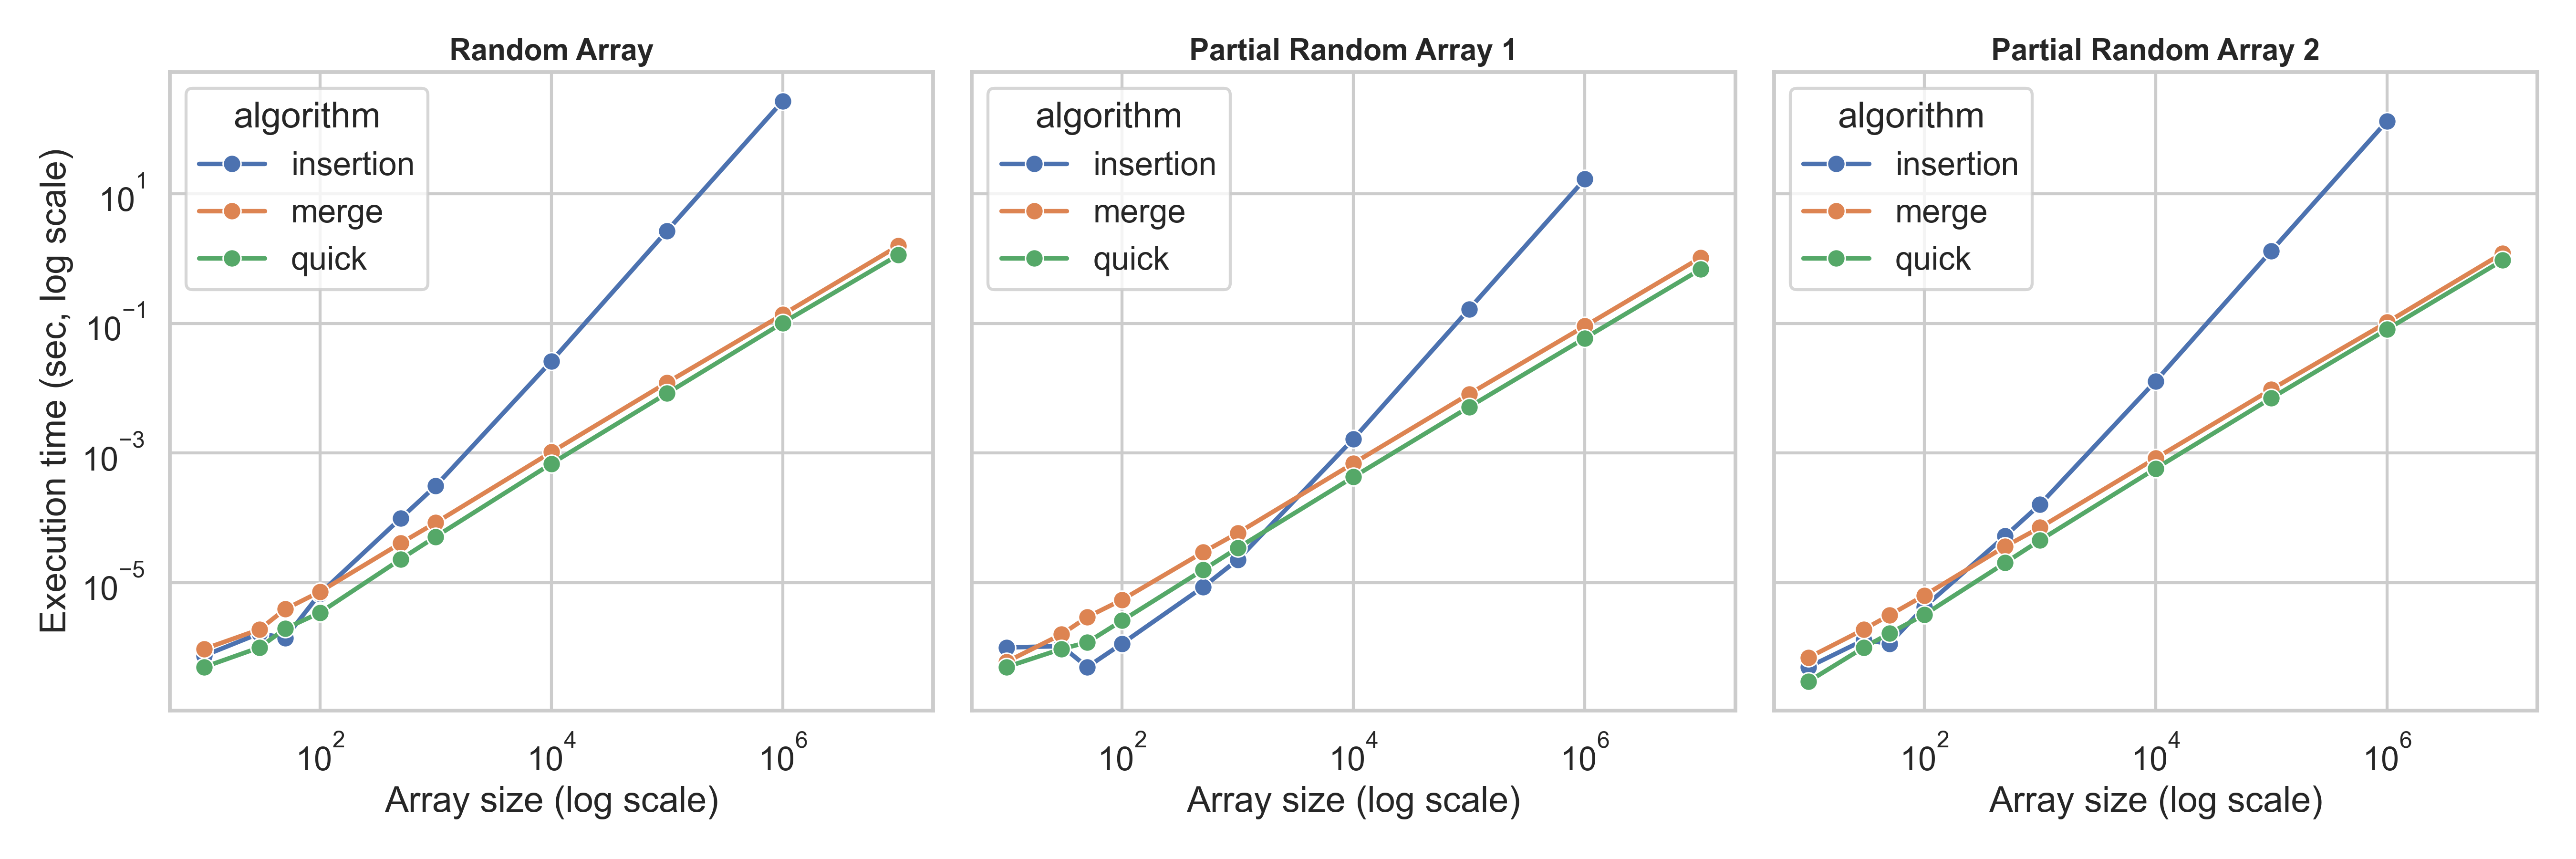
\includegraphics[width=\textwidth]{../bench/bench_result_base.png}
	\caption{Execution time comparison of insertion sort (the case of $10{,}000{,}000$ elements is omitted since the estimated runtime would exceed $7$ hours), merge sort, and quick sort on three input types. Both axes are shown in log scale. The complete benchmark table is available in Appendix~\ref{tab:bench-results}.}
	\label{fig:bench}
\end{figure}
\end{subq}

%%%%% C %%%%%
\begin{subq}{Let’s consider \code{random_array} data. Which algorithm is the best when the array size is small (e.g., 10, 30, 50). Explain why.}
\begin{answer}
\textbf{Insertion sort}\\
For small arrays the overhead of recursion in merge sort and quick sort is bigger than the actual work. Insertion sort is simple and very fast on small inputs so it wins here.
\end{answer}
\end{subq}

%%%%% D %%%%%
\begin{subq}{Let’s consider \code{random_array} data. Which algorithm becomes the eventually winner? Explain why.}
\begin{answer}
\textbf{Quick sort}\\
At one million elements quick sort takes about $0.10$ sec while merge sort takes $0.13$ sec and insertion sort takes $267$ sec. At ten million elements quick sort still leads with $1.13$ sec while merge sort takes $1.57$ sec. Quick sort becomes the winner for large random arrays.
\end{answer}
\end{subq}

%%%%% E %%%%%
\begin{subq}{Let’s consider the insertion sort algorithm. Which types of input arrays does insert sort have an advantage over other algorithms? Explain why.}
\begin{answer}
\textbf{Partial random arrays (1 \& 2)}\\
At one million elements insertion sort on random arrays takes $267$ sec but on partial random arrays it takes $16.7$ sec and $131$ sec. Insertion sort gains advantage when the data is already almost sorted because it needs only a small number of shifts.
\end{answer}
\end{subq}

%%%%% F %%%%%
\begin{subq}{Explain why quick sort is faster than merge sort.}
\begin{answer}
\textbf{in-place method}\\
Quick sort works in place so it avoids the extra memory overhead of merge sort. Its partition step creates smaller subproblems with less data movement than merging. The key factor is \textbf{pivot selection}. If the pivot splits the array fairly evenly the recursion depth is only $O(\log n)$ so the algorithm is very efficient. Choosing the last element or a random element makes quick sort probabilistically fast in practice but not strictly predictable.\\In the worst case where the pivot is always smallest or largest the runtime can degrade to $O(n^2)$ while merge sort stays at $O(n \log n)$.
\end{answer}
\end{subq}

%%%%% G %%%%%
\begin{subq}{Explain the advantages that merge sort has over quick sort.}
\begin{answer}
Quick sort depends on good pivot choice so the runtime is not always predictable. Merge sort always runs in $O(n \log n)$ time so the performance is consistent. It is stable so equal elements keep their original order which is useful in many cases. It also works well on linked lists and on external data because it uses sequential access.\\The tradeoff is that it needs extra memory while quick sort works in place.
\end{answer}
\end{subq}
\end{question_with_subs}

%%%%%%%%%%%%%%%%%%%%%%%%%%%%%%%%%%%%%%%%%%%%%
% Q5
%%%%%%%%%%%%%%%%%%%%%%%%%%%%%%%%%%%%%%%%%%%%%
\begin{question_with_subs}[5. Faster Merge Sort]{}
%%%%% A %%%%%
\begin{subq}{Implement the fast merge sort algorithm. The improved version divides the input array only until the size of the subarrays becomes less than 32. It then perform the insertion sort to conquer these small subarrays.}
\begin{lstlisting}[language=C, style=C]
#define THRESHOLD 32

void merge_sort_2(int arr[], int low, int high)
{
    if (high - low <= THRESHOLD) {
        insertion_sort(arr, low, high);
        return;
    }
    
    int mid = low + (high - low) / 2;
    merge_sort_2(arr, low, mid);
    merge_sort_2(arr, mid, high);
    merge(arr, low, mid, high);
}
\end{lstlisting}
\end{subq}

%%%%% B %%%%%
\begin{subq}{Compare the fast merge sort with its original one on the settings of problem 4.B.  Is performance improvement observable? Explain why it is faster.}
\begin{answer}
\textbf{Yes}. The fast merge sort is consistently faster across all input types.\\
From the data: at $n{=}1{,}000{,}000$, original merge sort takes $0.136$ sec on \code{random_array}, while fast merge sort takes $0.105$ sec.  
At $n{=}10{,}000{,}000$, the original is $1.57$ sec, but the fast version is $1.27$ sec.  
The reason is that the fast version switches to insertion sort when subarrays are below size $32$. Insertion sort runs very efficiently on these small (and nearly sorted) chunks, so recursion overhead is reduced.\\
Both algorithms remain $O(n \log n)$ in complexity, but the hybrid approach gains a practical speedup.
\end{answer}
\begin{figure}[h!]
	\centering
	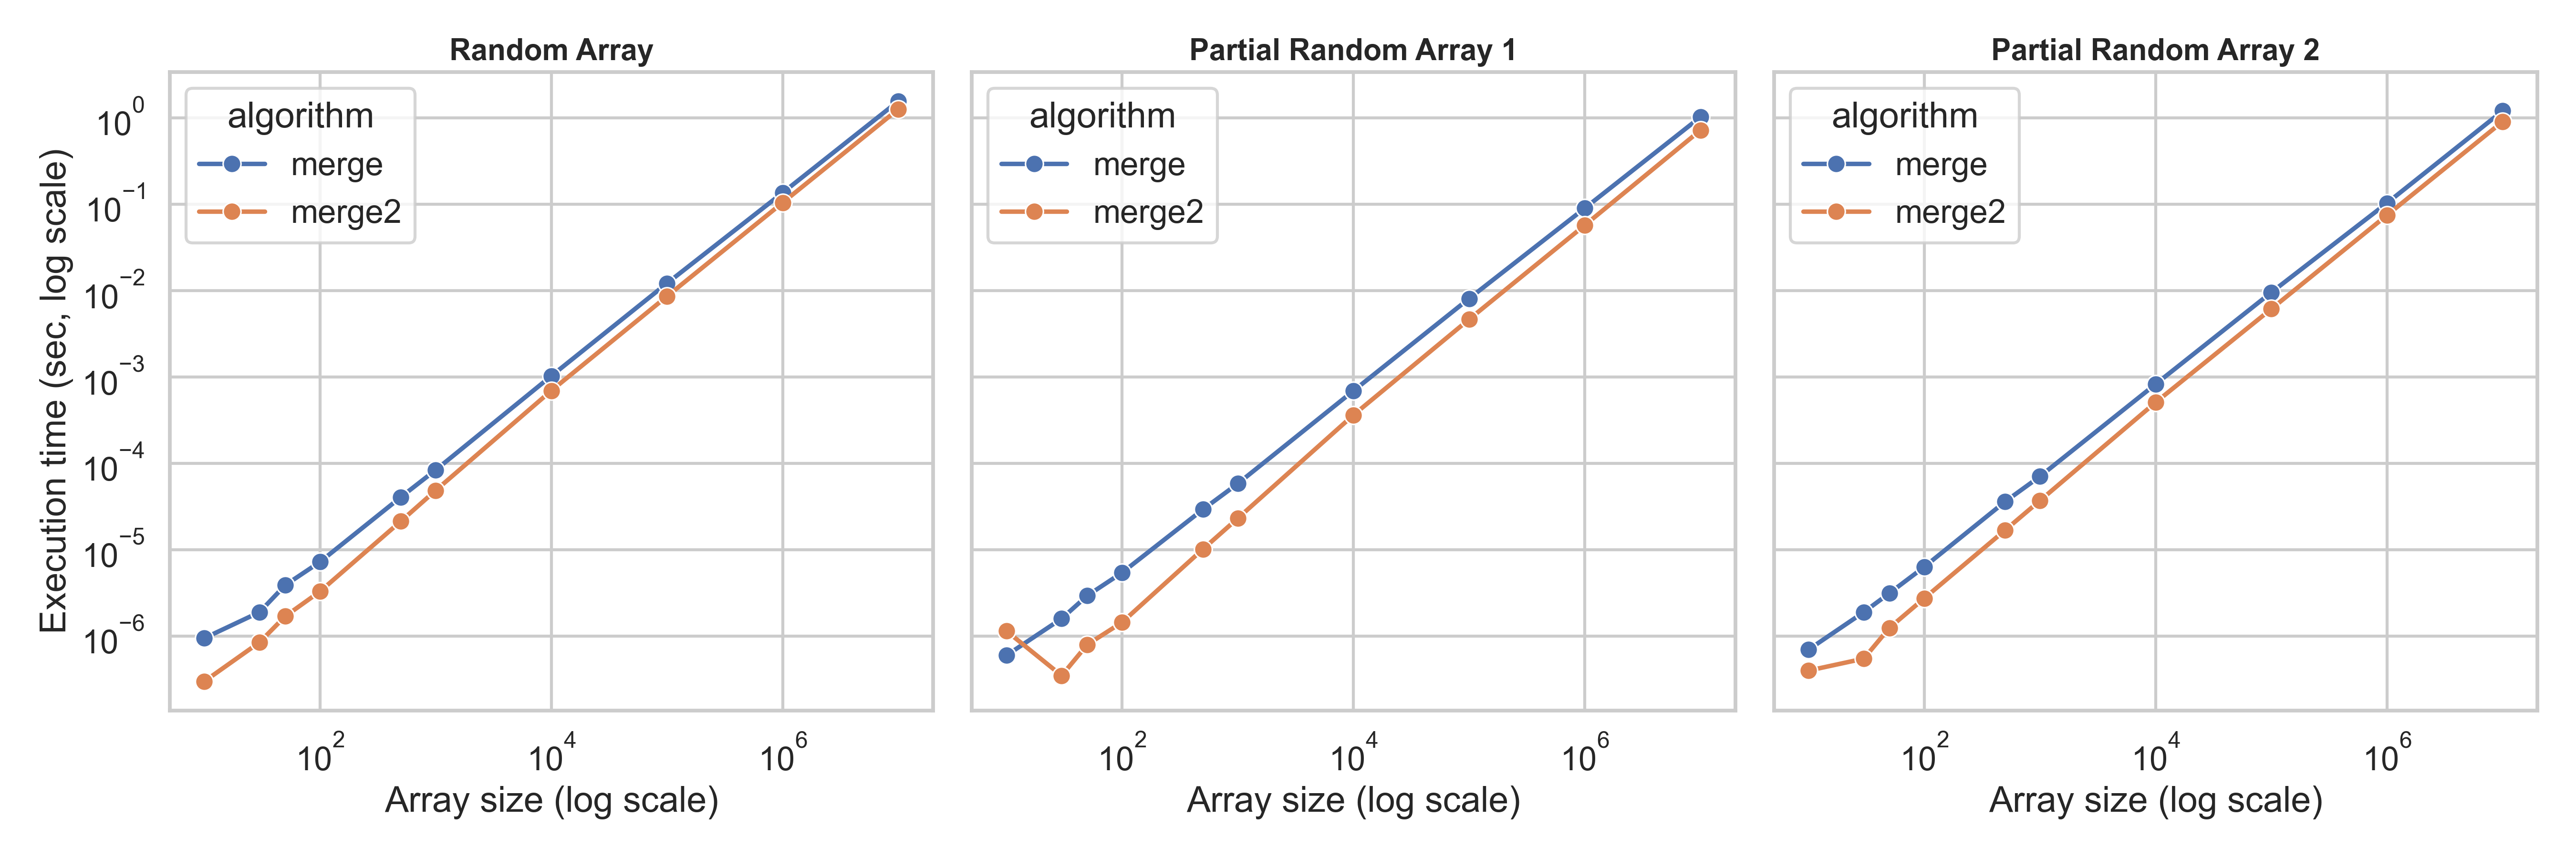
\includegraphics[width=\textwidth]{../bench/bench_result_faster_merge_1.png}
	\caption{Execution time comparison of original merge sort and fast merge sort. The fast version consistently outperforms the original by using insertion sort on small subarrays.}
\end{figure}
\end{subq}

%%%%% C %%%%%
\begin{subq}{Implement the faster merge sort algorithm by modifying the fast merge sort. This version first determine the necessity of merge operation before merging, and then skips the merge operation, when it is unnecessary.}
\begin{lstlisting}[language=C, style=C]
#define THRESHOLD 32

void merge_sort_3(int arr[], int low, int high)
{
    if (high - low <= THRESHOLD) {
        insertion_sort(arr, low, high);
        return;
    }
    
    int mid = low + (high - low) / 2;
    faster_merge_sort(arr, low, mid);
    faster_merge_sort(arr, mid, high);
    
    if (arr[mid - 1] > arr[mid]) {
        merge(arr, low, mid, high);
    }
}
\end{lstlisting}
\end{subq}

%%%%% D %%%%%
\begin{subq}{For which types of input array will this version produce performance improvements?. Explain why.}
\begin{answer}
\textbf{Partial random arrays (1 \& 2)}.\\
From the results: at $n{=}1{,}000{,}000$, merge3 takes only $0.025$ sec on \code{partial_random _array1} and $0.076$ sec on \code{partial_random_array2}, compared to $0.090$ sec and $0.103$ sec for the original merge.\\
The reason is that merge3 skips unnecessary merges. So on fully random arrays, improvements are smaller.
\end{answer}
\begin{figure}[h!]
	\centering
	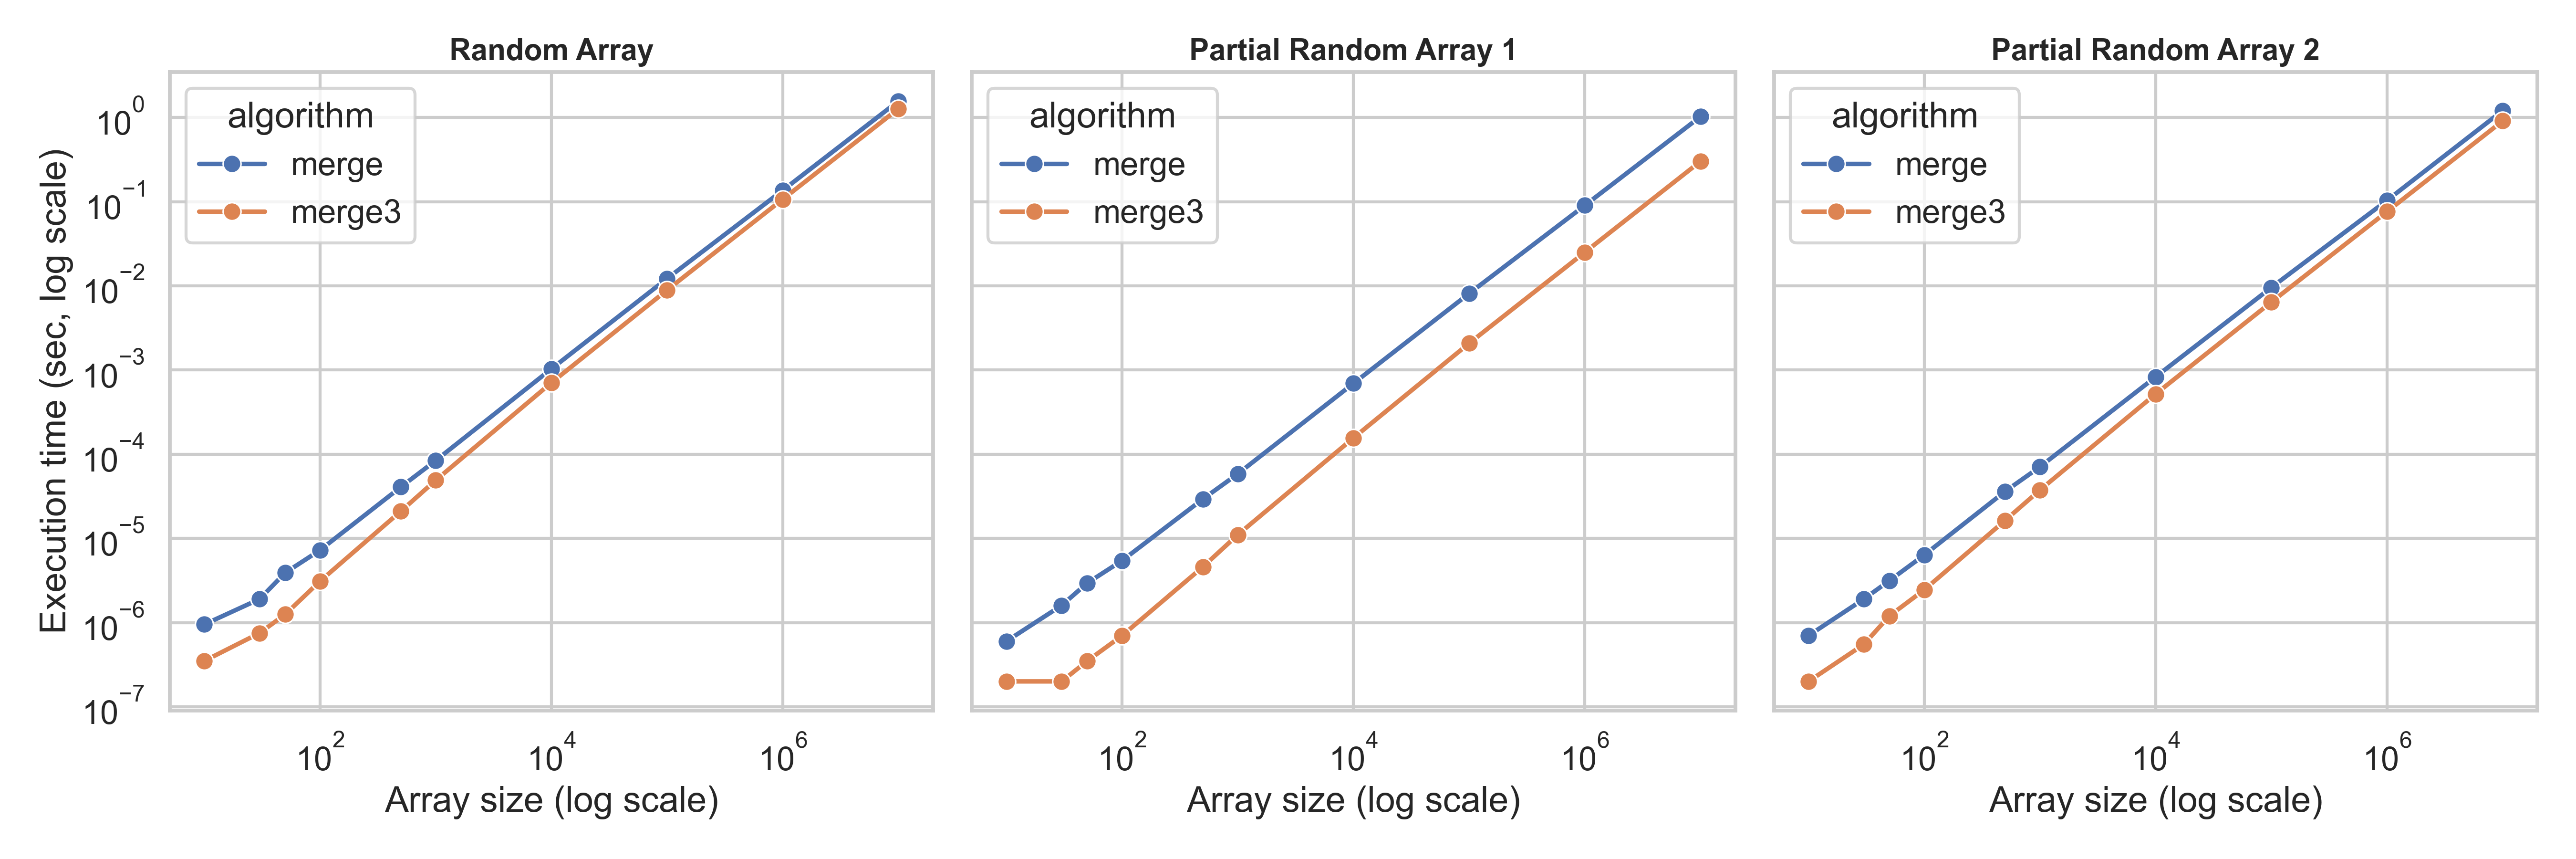
\includegraphics[width=\textwidth]{../bench/bench_result_faster_merge_2.png}
	\caption{Execution time comparison of original merge sort and optimized merge sort (merge3). The optimized version shows the largest improvement on partially sorted arrays by skipping unnecessary merges.}
	\label{fig:bench}
\end{figure}
\end{subq}
\end{question_with_subs}


\newpage
\appendix
\section*{\small Appendix}
\renewcommand{\arraystretch}{1}
\begin{table*}[h!]
\centering
\scriptsize
\begin{tabularx}{\textwidth}{l r X X X}
\toprule
\textbf{Algorithm} & \textbf{Size} & \textbf{Random Array} & \textbf{Partial Random 1} & \textbf{Partial Random 2} \\
\midrule
Insertion & $10$ & 0.00000075 & 0.00000100 & 0.00000050 \\
Insertion & $30$ & 0.00000165 & 0.00000105 & 0.00000130 \\
Insertion & $50$ & 0.00000140 & 0.00000050 & 0.00000115 \\
Insertion & $100$ & 0.00000680 & 0.00000115 & 0.00000420 \\
Insertion & $500$ & 0.00009885 & 0.00000855 & 0.00005225 \\
Insertion & $1{,}000$ & 0.00030985 & 0.00002265 & 0.00016035 \\
Insertion & $10{,}000$ & 0.02607045 & 0.00165270 & 0.01282990 \\
Insertion & $100{,}000$ & 2.67055610 & 0.16602390 & 1.30848705 \\
Insertion & $1{,}000{,}000$ & 267.85176080 & 16.72882800 & 131.53064900 \\
\midrule
Merge & $10$ & 0.00000095 & 0.00000060 & 0.00000070 \\
Merge & $30$ & 0.00000190 & 0.00000160 & 0.00000190 \\
Merge & $50$ & 0.00000390 & 0.00000295 & 0.00000315 \\
Merge & $100$ & 0.00000725 & 0.00000545 & 0.00000635 \\
Merge & $500$ & 0.00004080 & 0.00002940 & 0.00003615 \\
Merge & $1{,}000$ & 0.00008410 & 0.00005845 & 0.00007080 \\
Merge & $10{,}000$ & 0.00103160 & 0.00069455 & 0.00082880 \\
Merge & $100{,}000$ & 0.01220060 & 0.00812765 & 0.00955915 \\
Merge & $1{,}000{,}000$ & 0.13641800 & 0.09043000 & 0.10348600 \\
Merge & $10{,}000{,}000$ & 1.56927100 & 1.02761500 & 1.20692300 \\
\midrule
Merge2 & $10$ & 0.00000030 & 0.00000115 & 0.00000040 \\
Merge2 & $30$ & 0.00000085 & 0.00000035 & 0.00000055 \\
Merge2 & $50$ & 0.00000170 & 0.00000080 & 0.00000125 \\
Merge2 & $100$ & 0.00000330 & 0.00000145 & 0.00000275 \\
Merge2 & $500$ & 0.00002145 & 0.00001020 & 0.00001690 \\
Merge2 & $1{,}000$ & 0.00004880 & 0.00002320 & 0.00003715 \\
Merge2 & $10{,}000$ & 0.00069750 & 0.00036440 & 0.00050960 \\
Merge2 & $100{,}000$ & 0.00862670 & 0.00467135 & 0.00615385 \\
Merge2 & $1{,}000{,}000$ & 0.10478060 & 0.05743705 & 0.07488110 \\
Merge2 & $10{,}000{,}000$ & 1.26737810 & 0.72274165 & 0.90870235 \\
\midrule
Merge3 & $10$ & 0.00000035 & 0.00000020 & 0.00000020 \\
Merge3 & $30$ & 0.00000075 & 0.00000020 & 0.00000055 \\
Merge3 & $50$ & 0.00000125 & 0.00000035 & 0.00000120 \\
Merge3 & $100$ & 0.00000310 & 0.00000070 & 0.00000245 \\
Merge3 & $500$ & 0.00002105 & 0.00000460 & 0.00001635 \\
Merge3 & $1{,}000$ & 0.00004900 & 0.00001105 & 0.00003755 \\
Merge3 & $10{,}000$ & 0.00070610 & 0.00015615 & 0.00051895 \\
Merge3 & $100{,}000$ & 0.00891535 & 0.00208100 & 0.00641000 \\
Merge3 & $1{,}000{,}000$ & 0.10691445 & 0.02509835 & 0.07622190 \\
Merge3 & $10{,}000{,}000$ & 1.27277625 & 0.30195025 & 0.91110060 \\
\midrule
Quick & $10$ & 0.00000050 & 0.00000050 & 0.00000030 \\
Quick & $30$ & 0.00000100 & 0.00000095 & 0.00000100 \\
Quick & $50$ & 0.00000195 & 0.00000120 & 0.00000165 \\
Quick & $100$ & 0.00000345 & 0.00000260 & 0.00000320 \\
Quick & $500$ & 0.00002310 & 0.00001570 & 0.00002020 \\
Quick & $1{,}000$ & 0.00005120 & 0.00003435 & 0.00004505 \\
Quick & $10{,}000$ & 0.00068425 & 0.00042760 & 0.00057585 \\
Quick & $100{,}000$ & 0.00833690 & 0.00513570 & 0.00702175 \\
Quick & $1{,}000{,}000$ & 0.10170800 & 0.05907400 & 0.08065700 \\
Quick & $10{,}000{,}000$ & 1.13447600 & 0.68083100 & 0.93708000 \\
\bottomrule
\end{tabularx}
\caption{Full benchmark results: average execution time (sec) of sorting algorithms on different array sizes and input types.}
\label{tab:bench-results}
\end{table*}